\section{Aufbau}
\label{sec:Aufbau}
\begin{figure}
	\centering
	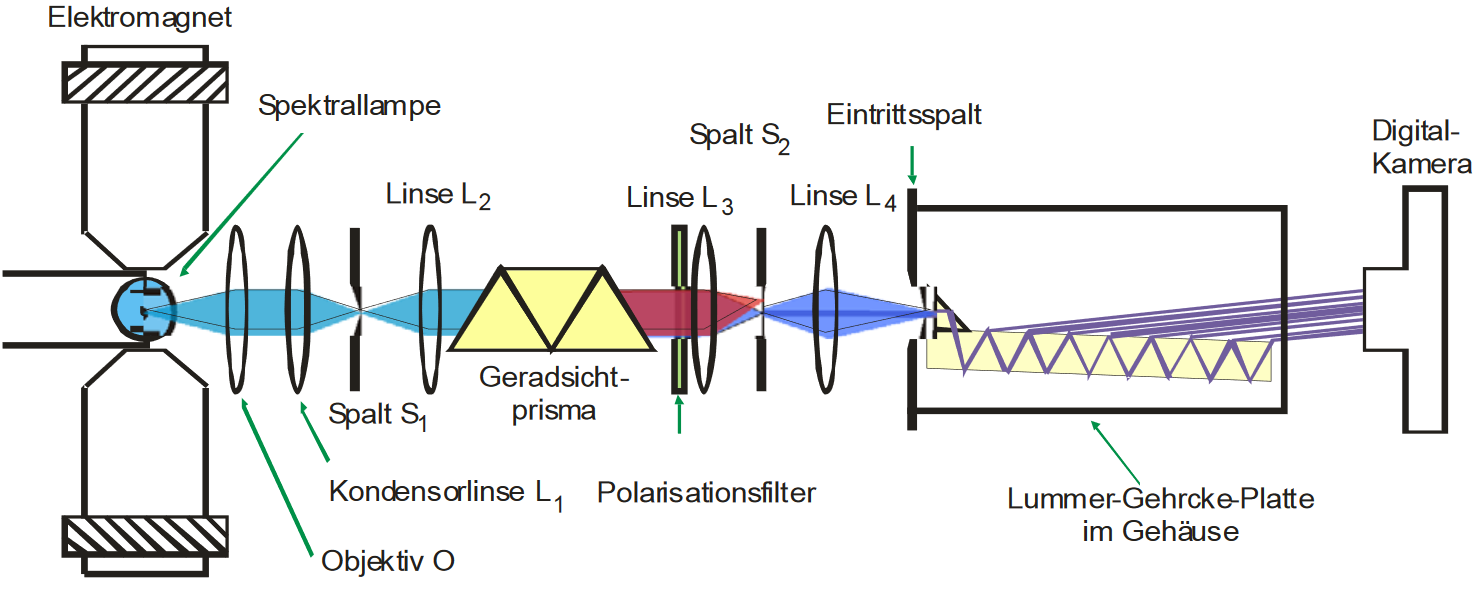
\includegraphics[width=\linewidth-50pt,height=\textheight-50pt,keepaspectratio]{content/Images/schema.png}
	\caption{Schematische Darstellung des experimentellen Aufbaus \cite{V27}.}
	\label{fig:schema}
\end{figure}

Zur Untersuchung des normalen bzw. anomalen Zeeman-Effektes wird als Spektrallampe eine Cadmium-Lampe verwendet. Diese wird mit Hilfe eines Elektromagneten einem Magnetfeld ausgesetzt. Das Bild dieser wird mit einem auf einer optischen Schiene befestigten Objektiv und einer Kondensorlinse scharf auf einen Spalt abgebildet. Das Licht, welches den Spalt passiert wird mit einer zweiten Linse parallelisiert, wobei darauf geachtet werden muss, dass das Lichtbündel nicht größer im Durchmesser als das darauf folgende Gradsichtprisma ist. In diesem werden die Spektrallinien der Cadmium-Lampe getrennt. In dem dahinter auf der optischen Schiene befestigten Polarisationsfilter kann gezielt eine Polarisationsrichtung heraus gefiltert werden. Das gefilterte Licht wird nun wieder mit einer Linse auf den nachfolgenden Spalt fokussiert. Am Spalt kann nun eine Spektrallinie ausgewählt werden, da diese aufgrund des Gradsichtprismas räumlich getrennt sind. Es wird die hell-blaue Spektrallinie zur Untersuchung des normalen Zeeman-Effektes und die rote Spektrallinie zur Untersuchung des anomalen Zeeman-Effektes verwendet. Mit Hilfe einer weiteren Linse wird das Lichtbündel scharf auf eine Lummer-Gehrcke-Platte fokussiert. Das entstehende Interferenzmuster wird mit einer Digitalkamera aufgenommen.